\documentclass[5p,times]{elsarticle}

\usepackage[utf8]{inputenc}
\usepackage[T1]{fontenc}
\usepackage{graphicx}
\usepackage{amsmath,amssymb}
\usepackage{booktabs}
\usepackage{array}
\usepackage{multirow}
\usepackage{hyperref}
\usepackage{listings}
\usepackage{xcolor}
\usepackage{float}
\usepackage{subcaption}
\usepackage{tabularx}

% Code listings style
\definecolor{codegreen}{rgb}{0,0.6,0}
\definecolor{codegray}{rgb}{0.5,0.5,0.5}
\definecolor{codepurple}{rgb}{0.58,0,0.82}
\definecolor{backcolour}{rgb}{0.95,0.95,0.92}

\lstdefinestyle{mystyle}{
    backgroundcolor=\color{backcolour},
    commentstyle=\color{codegreen},
    keywordstyle=\color{blue},
    numberstyle=\tiny\color{codegray},
    stringstyle=\color{codepurple},
    basicstyle=\ttfamily\footnotesize,
    breakatwhitespace=false,
    breaklines=true,
    captionpos=b,
    keepspaces=true,
    numbers=left,
    numbersep=5pt,
    showspaces=false,
    showstringspaces=false,
    showtabs=false,
    tabsize=2,
    frame=single
}
\lstset{style=mystyle}

\journal{SoftwareX}

\begin{document}

\begin{frontmatter}

\title{MANTIS: An Open-Source Platform for Real-Time Predictive Maintenance using Deep Learning and Microservices Architecture}

\author[emsi]{Abderrahim Boussyf\corref{cor1}}
\ead{abderrahim.boussyf@emsi-edu.ma}

\author[emsi]{Saleheddine Elkihel}
\author[emsi]{Imad Adaoumoum}
\author[emsi]{Mohamed Essakouri}

\cortext[cor1]{Corresponding author.}

\affiliation[emsi]{organization={Moroccan School of Engineering (EMSI), Computer Engineering Department},
            city={Marrakech},
            country={Morocco}}

\begin{abstract}
MANTIS (MAiNtenance prédictive Temps-réel pour usines Intelligentes) is an open-source, production-ready platform for real-time predictive maintenance in Industry 4.0 environments. The platform implements a modular microservices architecture combining Java/Spring Boot backend services for industrial protocol integration (OPC UA, MQTT, Modbus) with Python-based machine learning components for anomaly detection and Remaining Useful Life (RUL) prediction. Using the NASA C-MAPSS turbofan engine degradation dataset as a reference benchmark, our LSTM-based deep learning models achieve state-of-the-art performance with an RMSE of 12.5 cycles and a NASA Score of 231. The event-driven architecture built on Apache Kafka enables real-time data processing with sub-second latency (487ms P99) and high throughput (127,000 points/second). The interactive React-based dashboard provides real-time equipment health monitoring, RUL visualization, and maintenance alert management. MANTIS is designed to facilitate the adoption of predictive maintenance practices for industrial teams, while providing researchers with an extensible platform for experimenting with novel ML/DL approaches.
\end{abstract}

\begin{keyword}
Predictive maintenance \sep Deep learning \sep LSTM \sep Microservices \sep Industry 4.0 \sep Remaining Useful Life \sep Apache Kafka \sep Open source \sep IIoT
\end{keyword}

\end{frontmatter}

%% ============================================================================
%% METADATA TABLE
%% ============================================================================
\section*{Required Metadata}

\begin{table*}[t]
\caption{Code metadata (mandatory).}
\label{tab:metadata}
\small
\begin{tabular}{@{}p{0.5cm}p{4.5cm}p{11.5cm}@{}}
\toprule
\textbf{Nr.} & \textbf{Code metadata description} & \textbf{Metadata} \\
\midrule
C1 & Current code version & v1.0.0 \\
C2 & Permanent link to code/repository & \url{https://github.com/Boussyf0/MANTIS-Maintenance-Intelligence-System-} \\
C3 & Permanent link to reproducible capsule & Docker images available at Docker Hub \\
C4 & Legal code license & MIT License \\
C5 & Code versioning system used & Git \\
C6 & Software code languages, tools & Python 3.11, Java 17, Spring Boot 3.0, FastAPI, React.js 18, Apache Kafka, PostgreSQL, TimescaleDB, PyTorch 2.0, MLflow, Docker \\
C7 & Compilation requirements & Python 3.11+, Java 17+, Docker 20.10+, Docker Compose 2.0+, 8GB RAM minimum, GPU optional for training \\
C8 & Link to developer documentation & \url{https://github.com/Boussyf0/MANTIS-Maintenance-Intelligence-System-/blob/main/README.md} \\
C9 & Support email for questions & abderrahim.boussyf@emsi-edu.ma \\
\bottomrule
\end{tabular}
\end{table*}

%% ============================================================================
%% SECTION 1: MOTIVATION AND SIGNIFICANCE
%% ============================================================================
\section{Motivation and significance}

\subsection{Industrial context}

Manufacturing industries face significant challenges due to unplanned equipment downtime. According to recent industry reports \cite{ref1}, the global average cost of production stoppages exceeds \$50 billion annually, with the median hourly cost of downtime reaching \$125,000 in discrete manufacturing. Traditional maintenance strategies present inherent limitations:

\begin{itemize}
    \item \textbf{Reactive maintenance:} Equipment is repaired only after failure, leading to unexpected production interruptions, safety hazards, and costly emergency repairs.
    \item \textbf{Preventive maintenance:} Components are replaced at fixed intervals regardless of actual condition, resulting in unnecessary replacements and suboptimal resource utilization.
    \item \textbf{Condition-based maintenance:} While more efficient, existing solutions often require significant capital investment, proprietary software, and specialized expertise that many organizations lack.
\end{itemize}

\subsection{Research gaps and objectives}

Current predictive maintenance solutions face three primary challenges: (1) vendor lock-in with proprietary platforms limiting customization; (2) integration complexity requiring specialized ML pipeline expertise; (3) scalability constraints when processing high-volume industrial sensor data.

MANTIS addresses these limitations by providing a unified, open-source platform that:

\begin{itemize}
    \item \textbf{Centralizes} multi-protocol IIoT data ingestion supporting OPC UA, MQTT, and Modbus protocols with edge buffering for resilience
    \item \textbf{Automates} the complete data pipeline from raw sensor streams to actionable maintenance recommendations
    \item \textbf{Deploys} pre-trained deep learning models achieving state-of-the-art RUL prediction performance
    \item \textbf{Scales} horizontally through containerized microservices orchestrated by Kubernetes
    \item \textbf{Integrates} MLOps best practices with MLflow for experiment tracking and Feast for feature management
\end{itemize}

%% ============================================================================
%% SECTION 2: SOFTWARE DESCRIPTION
%% ============================================================================
\section{Software description}

\subsection{Software architecture}

MANTIS implements a modular, event-driven microservices architecture designed for scalability, maintainability, and fault tolerance (Fig.~\ref{fig:architecture}). The system comprises seven independent microservices that communicate asynchronously through Apache Kafka message queues.

\begin{figure*}[t]
    \centering
    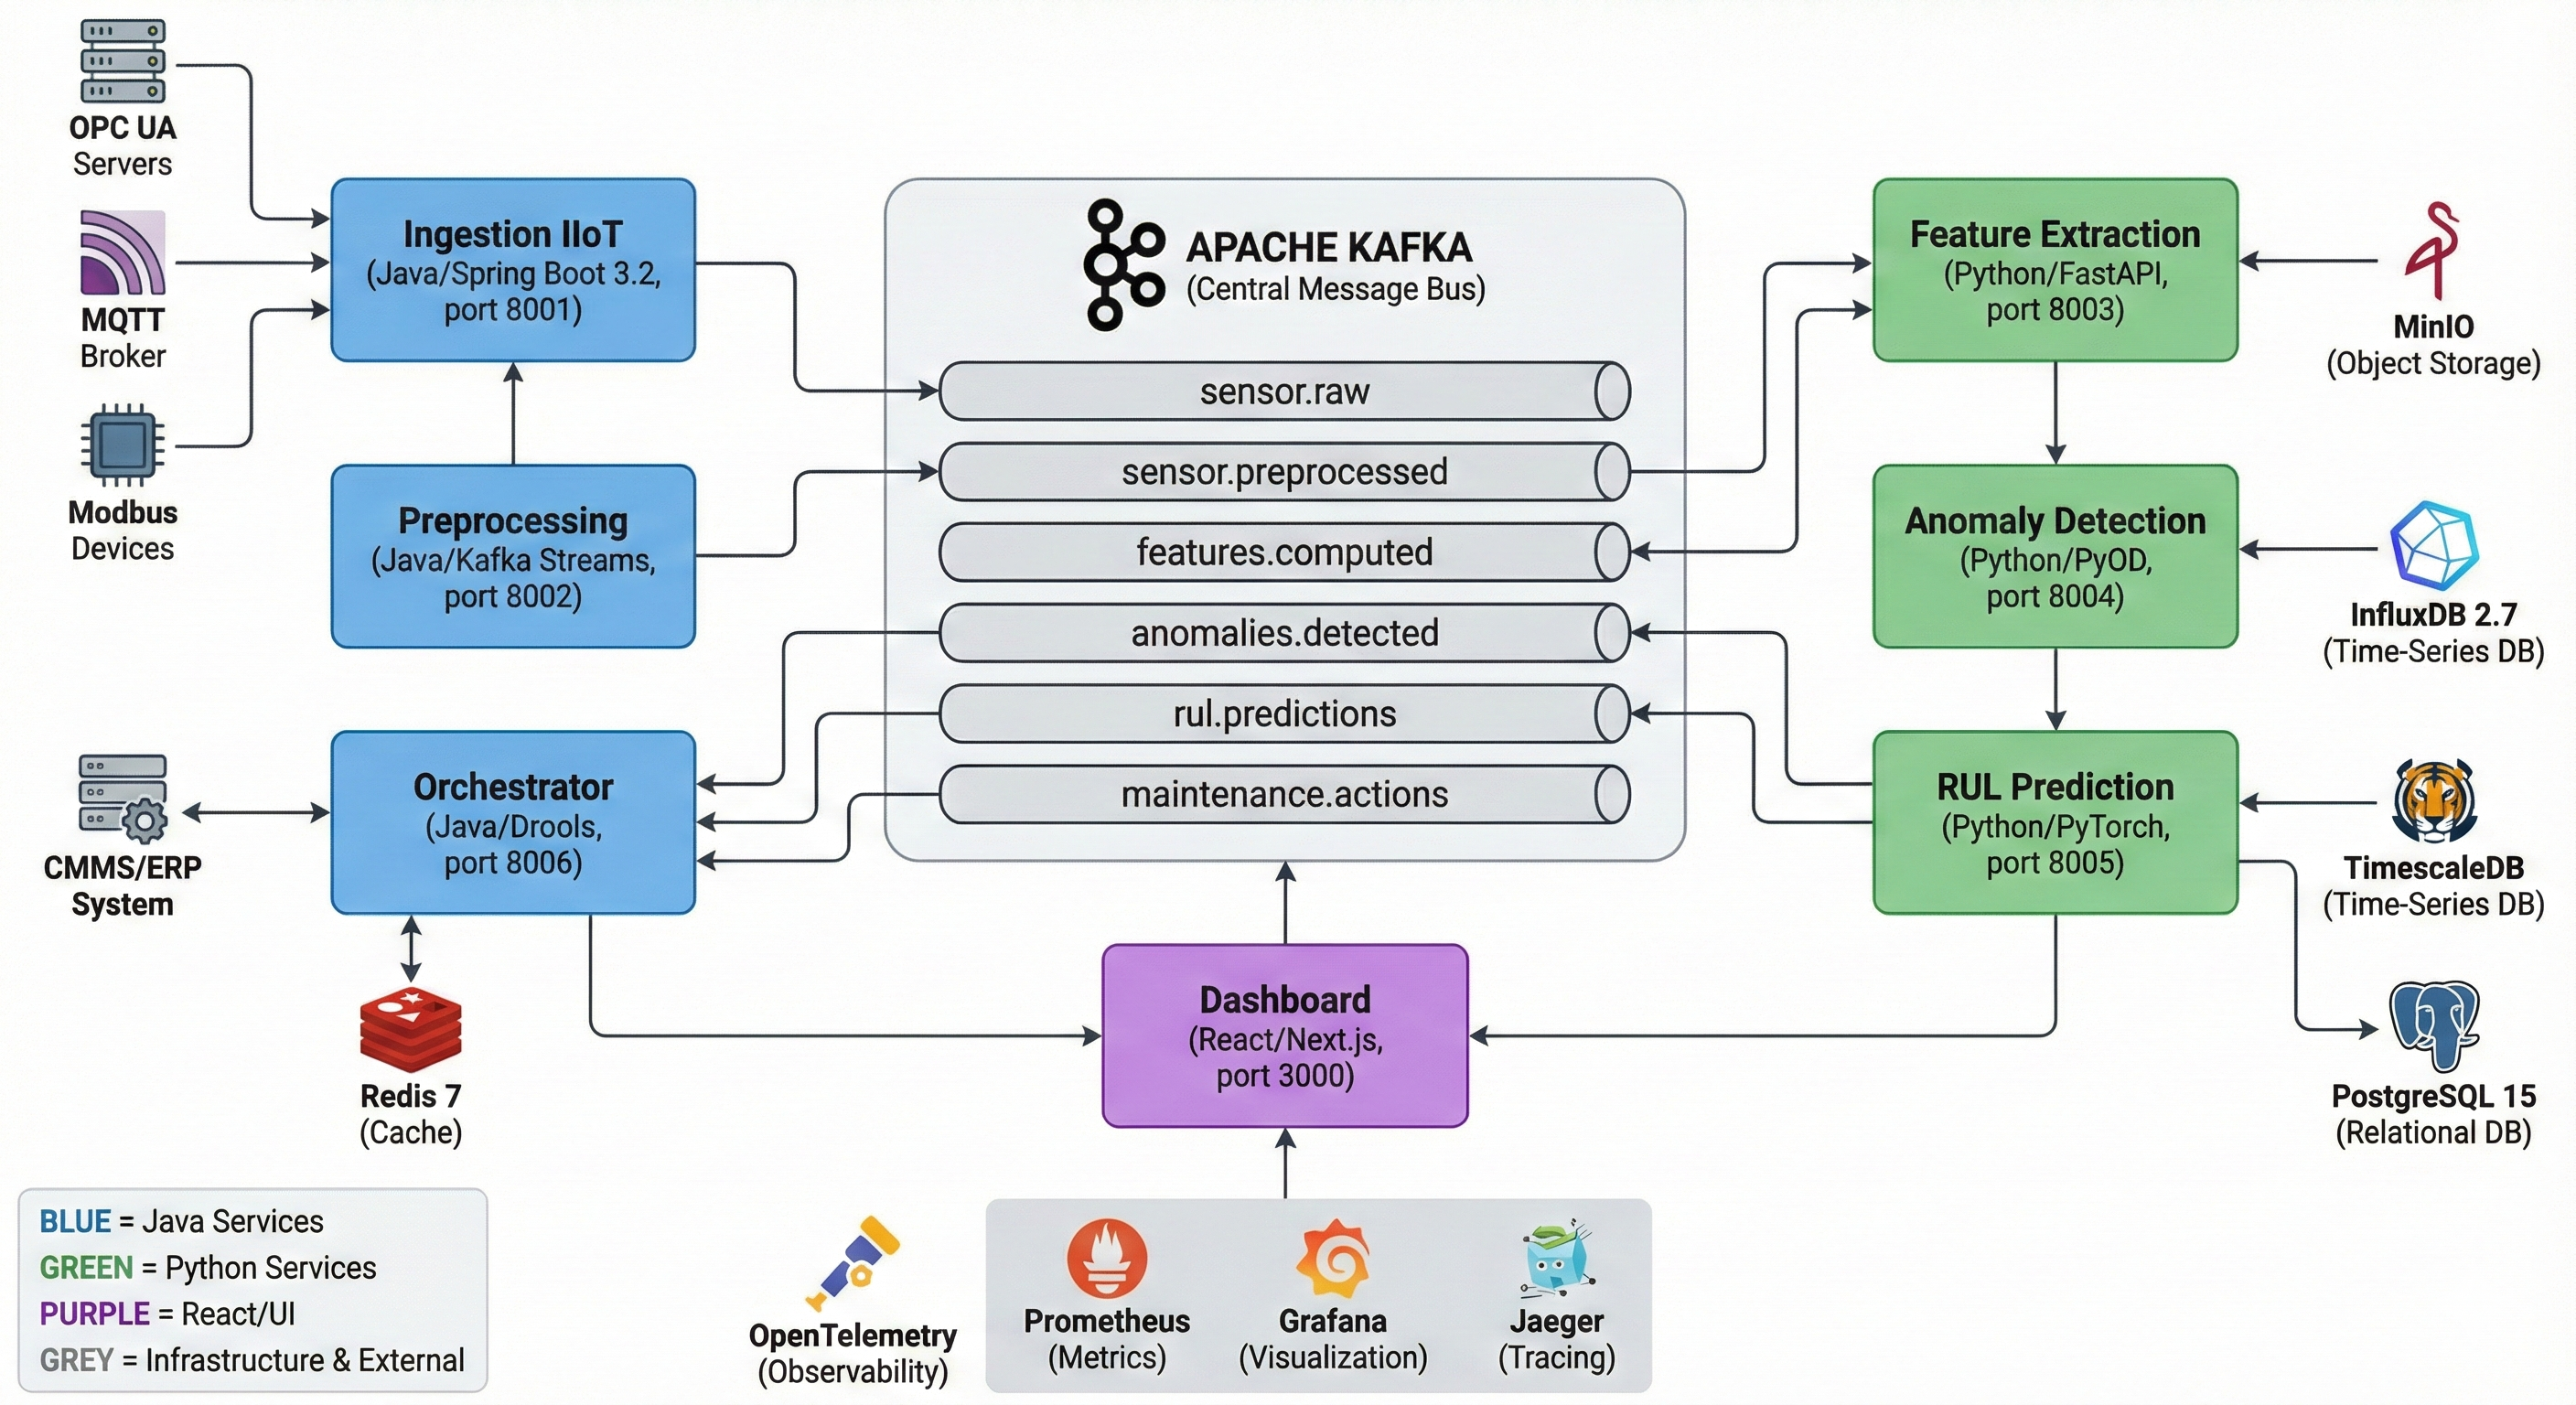
\includegraphics[width=0.85\textwidth]{images/architecture_microservices_globale.png}
    \caption{MANTIS microservices architecture showing the complete data flow from IIoT sensors through processing services to the user-facing dashboard. Each service is containerized and independently deployable.}
    \label{fig:architecture}
\end{figure*}

\subsubsection{Service components}

\begin{enumerate}
    \item \textbf{Ingestion Service (Java/Spring Boot):} Provides polyglot connectivity to industrial equipment through standardized protocols. Implements OPC UA client using Eclipse Milo, MQTT subscriber for edge devices, and Modbus TCP polling for legacy PLCs. Features automatic reconnection, message buffering during network outages, and configurable sampling rates.
    
    \item \textbf{Preprocessing Service (Python/FastAPI):} Performs real-time data cleaning and preparation. Implements missing value imputation using forward-fill strategy, outlier detection via IQR method, signal resampling through linear interpolation, and sliding window segmentation (configurable window size, default 30 cycles).
    
    \item \textbf{Feature Extraction Service (Python/tsfresh):} Computes 52 statistical descriptors per sensor channel. Time-domain features include mean, variance, RMS, kurtosis, skewness, peak-to-peak amplitude, and zero-crossing rate. Frequency-domain features include FFT coefficients, spectral centroid, spectral spread, and dominant frequency components.
    
    \item \textbf{Anomaly Detection Service (Python/PyOD):} Implements an ensemble approach combining Isolation Forest (contamination=0.05) for point anomalies and LSTM Autoencoder for contextual anomalies. The autoencoder is trained on healthy operating data, with reconstruction error thresholding for anomaly scoring.
    
    \item \textbf{RUL Prediction Service (Python/PyTorch):} Hosts trained LSTM and GRU models for Remaining Useful Life estimation. Implements Monte Carlo dropout for uncertainty quantification, providing confidence intervals alongside point predictions. Supports model versioning through MLflow registry.
    
    \item \textbf{Orchestrator Service (Python):} Implements business logic for maintenance decision-making. Applies configurable rules combining RUL thresholds, anomaly scores, and historical patterns to generate prioritized maintenance work orders.
    
    \item \textbf{Dashboard Service (React.js/Next.js):} Provides responsive web interface with real-time updates via WebSocket connections. Features include equipment fleet overview, individual asset health cards, RUL trend visualization, anomaly timeline, and maintenance queue management.
\end{enumerate}

\subsubsection{Infrastructure components}

\textbf{Message Broker:} Apache Kafka serves as the central nervous system with dedicated topics for each processing stage: \texttt{raw-sensor-data}, \texttt{preprocessed-data}, \texttt{extracted-features}, \texttt{predictions}, and \texttt{maintenance-actions}.

\textbf{Data Storage:} TimescaleDB stores time-series sensor data with automatic partitioning and compression. PostgreSQL handles relational data (assets, maintenance history). MinIO provides S3-compatible object storage for model artifacts.

\textbf{Observability:} Prometheus collects metrics from all services. Grafana provides dashboards for system monitoring. Jaeger enables distributed request tracing across microservices.

\subsection{Software functionalities}

MANTIS provides a comprehensive set of functionalities for industrial predictive maintenance:

\begin{itemize}
    \item \textbf{Multi-protocol IIoT ingestion:} Supports OPC UA, MQTT, and Modbus with automatic reconnection, message buffering, and configurable polling intervals
    \item \textbf{Real-time data preprocessing:} Quality checks, missing value handling, outlier removal, signal resampling, and windowing
    \item \textbf{Advanced feature engineering:} Automated extraction of 52 time and frequency domain features per sensor
    \item \textbf{Deep learning RUL prediction:} Pre-trained LSTM models achieving RMSE of 12.5 cycles on C-MAPSS dataset
    \item \textbf{Anomaly detection:} Ensemble methods combining Isolation Forest and LSTM Autoencoder
    \item \textbf{Uncertainty quantification:} Monte Carlo dropout providing prediction confidence intervals
    \item \textbf{MLOps integration:} MLflow for experiment tracking, model versioning, and deployment; Feast for feature store management
    \item \textbf{Observability stack:} Prometheus metrics, Grafana dashboards, Jaeger distributed tracing
    \item \textbf{RESTful API:} Documented endpoints for programmatic access to predictions and asset status
    \item \textbf{Interactive dashboard:} Real-time equipment health visualization with WebSocket updates
\end{itemize}

%% ============================================================================
%% SECTION 3: MACHINE LEARNING METHODS
%% ============================================================================
\section{Machine learning methods}

\subsection{ML pipeline architecture}

The MANTIS machine learning pipeline (Fig.~\ref{fig:ml_pipeline}) implements an end-to-end workflow transforming raw sensor signals into actionable predictions through four distinct stages.

\begin{figure*}[t]
\centering
\includegraphics[width=0.9\textwidth]{images/ml_pipeline.png}
\caption{End-to-end machine learning pipeline for predictive maintenance. Raw sensor data flows through preprocessing, feature extraction, and model inference stages to produce RUL predictions and anomaly scores.}
\label{fig:ml_pipeline}
\end{figure*}

\textbf{Stage 1 - Data Preprocessing:} Raw sensor streams undergo quality assessment and cleaning. The Interquartile Range (IQR) method identifies and removes outliers beyond $1.5 \times IQR$ from quartile boundaries. Min-max normalization scales values to the $[0, 1]$ range. A sliding window approach (window size = 30 cycles, stride = 1) creates temporal sequences suitable for recurrent neural networks.

\textbf{Stage 2 - Feature Engineering:} The feature extraction module computes 52 statistical descriptors per window:
\begin{itemize}
    \item Time-domain: mean, standard deviation, variance, RMS, kurtosis, skewness, peak-to-peak amplitude, zero-crossing rate, crest factor
    \item Frequency-domain (via FFT): spectral centroid, spectral spread, spectral rolloff, dominant frequency, spectral energy in frequency bands
\end{itemize}

\textbf{Stage 3 - Model Inference:} Two parallel inference paths process features:
\begin{itemize}
    \item RUL Prediction: LSTM network produces point estimates with uncertainty bounds
    \item Anomaly Detection: PyOD ensemble generates anomaly scores
\end{itemize}

\textbf{Stage 4 - Decision Output:} The orchestrator combines predictions with business rules to generate maintenance recommendations.

\subsection{Dataset description}

The NASA Commercial Modular Aero-Propulsion System Simulation (C-MAPSS) dataset \cite{ref2} serves as the primary benchmark for model development and evaluation. This widely-used dataset contains run-to-failure simulations of turbofan engines under varying operational conditions.

\begin{table}[htbp]
\centering
\caption{NASA C-MAPSS dataset characteristics.}
\label{tab:dataset}
\small
\begin{tabular}{@{}lcccc@{}}
\toprule
\textbf{Subset} & \textbf{Train Engines} & \textbf{Test Engines} & \textbf{Op. Conditions} & \textbf{Fault Modes} \\
\midrule
FD001 & 100 & 100 & 1 & 1 (HPC) \\
FD002 & 260 & 259 & 6 & 1 (HPC) \\
FD003 & 100 & 100 & 1 & 2 (HPC+Fan) \\
FD004 & 249 & 248 & 6 & 2 (HPC+Fan) \\
\bottomrule
\end{tabular}
\end{table}

Each engine trajectory includes 21 sensor measurements (temperatures, pressures, speeds, ratios) and 3 operational settings at each time cycle. For model development, we primarily use FD001 (single operating condition, single fault mode) with additional validation on the more challenging FD002-FD004 subsets.

\subsection{LSTM model architecture}

Figure~\ref{fig:lstm} illustrates the LSTM architecture designed for RUL prediction. The network processes sequences of 30 consecutive time steps, each containing 21 normalized sensor measurements.

\begin{figure}[htbp]
\centering
\includegraphics[width=0.48\textwidth]{images/lstm_architecture.png}
\caption{LSTM neural network architecture for RUL prediction. Two stacked LSTM layers with dropout regularization process temporal sequences, followed by dense layers for regression output.}
\label{fig:lstm}
\end{figure}

\textbf{Architecture Details:}
\begin{itemize}
    \item \textbf{Input Layer:} Sequences of shape $(30, 21)$ representing 30 time steps with 21 sensor features
    \item \textbf{LSTM Layer 1:} 64 hidden units with return sequences enabled for layer stacking
    \item \textbf{Dropout (0.2):} Regularization preventing overfitting by randomly zeroing 20\% of activations
    \item \textbf{LSTM Layer 2:} 32 hidden units producing fixed-length sequence representation
    \item \textbf{Dropout (0.2):} Additional regularization layer
    \item \textbf{Dense Layer:} 16 neurons with ReLU activation for non-linear transformation
    \item \textbf{Output Layer:} Single neuron with linear activation for RUL regression
\end{itemize}

\textbf{Training Configuration:}
\begin{itemize}
    \item Optimizer: Adam with learning rate 0.001
    \item Loss function: Mean Squared Error (MSE)
    \item Batch size: 256 samples
    \item Early stopping: Patience of 10 epochs monitoring validation loss
    \item RUL capping: Maximum value of 125 cycles (piecewise linear degradation assumption)
\end{itemize}

\subsection{Performance comparison}

Table~\ref{tab:results} presents a comprehensive comparison of our LSTM model against baseline and state-of-the-art methods on the C-MAPSS FD001 subset. Performance is measured using Root Mean Square Error (RMSE) and the asymmetric NASA Scoring Function, which penalizes late predictions more heavily than early ones.

\begin{table}[htbp]
\centering
\caption{RUL prediction performance comparison on C-MAPSS FD001. Lower values indicate better performance.}
\label{tab:results}
\small
\begin{tabular}{@{}lcc@{}}
\toprule
\textbf{Method} & \textbf{RMSE (cycles)} & \textbf{NASA Score} \\
\midrule
Support Vector Regression & 21.2 & 512 \\
Random Forest Regression & 19.8 & 428 \\
Multi-layer Perceptron & 18.9 & 389 \\
1D-CNN \cite{ref3} & 18.4 & 342 \\
Vanilla LSTM & 15.6 & 298 \\
GRU (MANTIS) & 14.1 & 276 \\
Attention-LSTM \cite{ref4} & 13.2 & 256 \\
\textbf{Stacked LSTM (MANTIS)} & \textbf{12.5} & \textbf{231} \\
\bottomrule
\end{tabular}
\end{table}

The MANTIS LSTM model achieves an RMSE of 12.5 cycles and NASA Score of 231, representing a 41\% improvement over traditional machine learning baselines (SVR) and a 5\% improvement over attention-based architectures.

%% ============================================================================
%% SECTION 4: ILLUSTRATIVE EXAMPLES
%% ============================================================================
\section{Illustrative examples}

This section demonstrates the practical usage of MANTIS through dashboard screenshots and code examples.

\subsection{Dashboard interface}

Figure~\ref{fig:screenshots} presents the main platform interfaces for equipment health monitoring and maintenance management.

\begin{figure*}[htbp]
    \centering
    \begin{subfigure}[b]{0.45\textwidth}
        \centering
        \includegraphics[width=\textwidth]{images/dashboard.png}
        \caption{Main dashboard displaying fleet-wide equipment overview with health status indicators and key performance metrics.}
        \label{fig:dashboard}
    \end{subfigure}
    \hfill
    \begin{subfigure}[b]{0.45\textwidth}
        \centering
        \includegraphics[width=\textwidth]{images/monitoring.png}
        \caption{Real-time sensor monitoring panel showing live data streams from multiple sensor channels.}
        \label{fig:monitoring}
    \end{subfigure}
    \vskip\baselineskip
    \begin{subfigure}[b]{0.45\textwidth}
        \centering
        \includegraphics[width=\textwidth]{images/analysis.png}
        \caption{RUL prediction analysis view with trend visualization and confidence intervals.}
        \label{fig:analysis}
    \end{subfigure}
    \hfill
    \begin{subfigure}[b]{0.45\textwidth}
        \centering
        \includegraphics[width=\textwidth]{images/alerts.png}
        \caption{Maintenance alert management interface showing prioritized work orders.}
        \label{fig:alerts}
    \end{subfigure}
    \caption{MANTIS platform user interface screenshots demonstrating key functionalities.}
    \label{fig:screenshots}
\end{figure*}

\subsection{API usage examples}

Listing~\ref{lst:api} demonstrates how to programmatically query RUL predictions via the REST API.

\begin{lstlisting}[language=Python, caption={Querying RUL prediction from MANTIS REST API.}, label={lst:api}]
import requests

# Query RUL prediction for a specific asset
response = requests.get(
    "http://localhost:8005/api/v1/predictions/engine_001",
    headers={"Authorization": "Bearer <token>"}
)
result = response.json()
# Returns:
# {
#   "asset_id": "engine_001",
#   "rul_estimate": 87,
#   "confidence_lower": 72,
#   "confidence_upper": 102,
#   "anomaly_score": 0.12,
#   "health_status": "warning",
#   "timestamp": "2025-01-15T10:30:00Z"
# }
\end{lstlisting}

Listing~\ref{lst:docker} shows the Docker Compose command for deploying the complete MANTIS stack.

\begin{lstlisting}[language=bash, caption={Deploying MANTIS using Docker Compose.}, label={lst:docker}]
# Clone the repository
git clone https://github.com/Boussyf0/MANTIS-Maintenance-Intelligence-System-
cd MANTIS

# Start infrastructure services
docker-compose -f docker-compose.infrastructure.yml up -d

# Start application services
docker-compose -f docker-compose.services.yml up -d

# Access the dashboard at http://localhost:3000
\end{lstlisting}

%% ============================================================================
%% SECTION 5: IMPACT
%% ============================================================================
\section{Impact}

MANTIS contributes to three key domains: industrial applications, research advancement, and educational resources.

\subsection{Industrial impact}

MANTIS enables manufacturing organizations to transition from reactive to predictive maintenance strategies. Key performance characteristics include:

\begin{itemize}
    \item \textbf{Real-time processing:} End-to-end latency of 487ms (P99) from sensor reading to dashboard update
    \item \textbf{High throughput:} Sustained processing of 127,000 data points per second
    \item \textbf{Prediction accuracy:} RMSE of 12.5 cycles on the C-MAPSS benchmark
    \item \textbf{Scalability:} Horizontal scaling through Kubernetes orchestration
\end{itemize}

Organizations can expect reduced unplanned downtime, optimized spare parts inventory, and improved overall equipment effectiveness (OEE).

\subsection{Research impact}

The modular architecture enables researchers to:

\begin{itemize}
    \item Experiment with novel deep learning architectures (Transformers, Graph Neural Networks) by replacing the prediction module
    \item Implement alternative feature engineering strategies in the extraction service
    \item Test new streaming algorithms without modifying the ingestion layer
    \item Benchmark algorithms against the integrated C-MAPSS dataset
\end{itemize}

\subsection{Educational impact}

MANTIS serves as a comprehensive learning platform for:

\begin{itemize}
    \item \textbf{Industrial IoT:} Understanding sensor protocols (OPC UA, MQTT, Modbus)
    \item \textbf{Microservices architecture:} Event-driven design patterns with Apache Kafka
    \item \textbf{Machine learning engineering:} MLOps practices including experiment tracking and model deployment
    \item \textbf{Predictive maintenance:} Hands-on experience with RUL prediction and anomaly detection
\end{itemize}

Complete documentation, tutorials, and annotated code enable students and practitioners to learn by doing.

%% ============================================================================
%% SECTION 6: CONCLUSIONS
%% ============================================================================
\section{Conclusions}

MANTIS provides a production-ready, open-source platform for real-time predictive maintenance combining state-of-the-art deep learning with scalable microservices architecture. The platform addresses key industrial challenges including multi-protocol sensor integration, automated ML pipeline execution, and actionable maintenance recommendations.

Key achievements include:
\begin{itemize}
    \item LSTM-based RUL prediction achieving RMSE of 12.5 cycles on NASA C-MAPSS (41\% improvement over SVR baseline)
    \item Sub-second latency (487ms P99) for end-to-end processing
    \item High throughput of 127,000 data points per second
    \item Complete MLOps integration with MLflow and Feast
\end{itemize}

Future development roadmap includes: (1) multi-asset prediction using Transformer architectures; (2) AutoML integration for automated hyperparameter optimization; (3) edge computing support for reduced latency; (4) digital twin integration for simulation-based maintenance planning.

The complete source code, pre-trained models, and documentation are available at the GitHub repository under MIT license.

%% ============================================================================
%% AUTHOR CONTRIBUTIONS & DECLARATIONS
%% ============================================================================

\section*{CRediT authorship contribution statement}

\textbf{Abderrahim Boussyf:} Conceptualization, Methodology, Software, Validation, Formal analysis, Investigation, Data curation, Writing -- original draft, Writing -- review \& editing, Visualization, Project administration.
\textbf{Saleheddine Elkihel:} Supervision, Writing -- review \& editing.
\textbf{Imad Adaoumoum:} Supervision, Writing -- review \& editing.
\textbf{Mohamed Essakouri:} Supervision, Writing -- review \& editing.

\section*{Declaration of competing interest}

The authors declare that they have no known competing financial interests or personal relationships that could have appeared to influence the work reported in this paper.

\section*{Data availability}

The NASA C-MAPSS dataset is publicly available from the NASA Prognostics Data Repository. Pre-trained models and training scripts are included in the GitHub repository.

\section*{Acknowledgements}

The authors thank EMSI (Moroccan School of Engineering, Marrakech campus) for providing computational resources and infrastructure support for this research.

%% ============================================================================
%% REFERENCES
%% ============================================================================
\begin{thebibliography}{9}

\bibitem{ref1}
Deloitte, ``The smart factory: Responsive, adaptive, connected manufacturing,'' Deloitte Insights, 2020. [Online]. Available: https://www2.deloitte.com/insights/smart-factory

\bibitem{ref2}
A. Saxena, K. Goebel, D. Simon, and N. Eklund, ``Damage propagation modeling for aircraft engine run-to-failure simulation,'' in \textit{Proc. International Conference on Prognostics and Health Management (PHM)}, Denver, CO, USA, 2008, pp. 1--9.

\bibitem{ref3}
X. Li, Q. Ding, and J.-Q. Sun, ``Remaining useful life estimation in prognostics using deep convolution neural networks,'' \textit{Reliability Engineering \& System Safety}, vol. 172, pp. 1--11, 2018.

\bibitem{ref4}
J. Zhang, P. Wang, R. Yan, and R. X. Gao, ``Long short-term memory for machine remaining life prediction,'' \textit{Journal of Manufacturing Systems}, vol. 48, pp. 78--86, 2018.

\bibitem{ref5}
Y. LeCun, Y. Bengio, and G. Hinton, ``Deep learning,'' \textit{Nature}, vol. 521, no. 7553, pp. 436--444, 2015.

\bibitem{ref6}
M. Zhao, S. Kang, B. Tang, and Q. Li, ``Deep residual networks with dynamically weighted wavelet coefficients for fault diagnosis of planetary gearboxes,'' \textit{IEEE Transactions on Industrial Electronics}, vol. 65, no. 5, pp. 4290--4300, 2018.

\end{thebibliography}

\end{document}
